% -*- root: 00-main.tex -*-
\section{Methods}
\label{sec:methods}
%
\subsection{Related work}
\label{sec:methods_background}
Registration-segmentation methods are typically built including a deformation
  model to guide the evolution of a segmentation algorithm.
Even though some Bayesian approaches have been proposed to solve the joint problem
  \citep{wyatt_map_2003}, segmentation is usually performed using an evolving
  active contour \citep{chan_active_2001} that normally includes a shape prior
  term to the energy functional \citep{chen_using_2002,bresson_variational_2006,
  chan_level_2005,cremers_kernel_2006,gastaud_combining_2004}.
These methods generally have an explicit description of the expected relative boundary
  locations of the object to be delineated, and some, even model the statistical deviations
  from this average shape.


An early ``morphing''-segmentation approach was proposed in \citep{bertalmio_morphing_2000},
  and the first proper registration method was presented by \citeauthor{yezzi_variational_2001}
  \citep{yezzi_variational_2001}, where the energy functional is defined simultaneously in the target
  and reference images with an affine transformation supporting the coordinates mapping
  (the so-called ``2 \glspl*{pde} approach'').
\citeauthor{vemuri_joint_2003} proposed the first atlas-based registration \citep{vemuri_joint_2003}
  based on the level-sets framework and using only one \gls*{pde}.
The principal application of these techniques was the image registration between timesteps in
  a time-series or between different images \citep{paragios_level_2003}.
\citeauthor{unal_coupled_2005} \citep{unal_coupled_2005} extended the idea of
  \citep{bertalmio_morphing_2000,yezzi_variational_2001} to nonlinear registration
  using a free deformation field model.
A summary of these second set of techniques is performed in \citep{droske_mumfordshah_2009},
  proposing two different approaches to applying the Mumford-Shah \citep{mumford_optimal_1989}
  functional in joint registration and segmentation, through the propagation of the deformation
  field from the contours to the whole image definition.
Finally, \citeauthor{gorthi_active_2011} presented a comprehensive generalization of the
  existing methodologies \citep{gorthi_active_2011} based on the level-sets approximation.
Even though the historical evolution of joint segmentation and registration procedures is strongly
  linked to the level sets approximation, our work is based in derivations of the \acrlong{acwe}
  framework \citep{chan_active_2001}, and related to \citep{guyader_combined_2011}.


Finally, a derivation of the latter group is composed by atlas-based segmentation methods
  \citep{gorthi_segmentation_2009,gorthi_active_2011,pohl_unifying_2005,pohl_bayesian_2006,
  wang_joint_2006}, where the prior imposes consistent voxel-based classification of contiguous
  regions.
A comprehensive summary of the methodologies derived from the \acrlong{acwe} model, with special attention
  to joint registration-segmentation methods is found in \citep{gorthi_active_2011}.

\subsection{Cost-function derivation}
\label{sec:methods_map}

In a Bayesian framework, the mappings $U$ in \autoref{eq:transform} are
  evaluated based on their posterior probability given the observed data
  $R$.
Using the Bayes' rule, the posterior likelihood is computed as:
  \begin{equation}
  P(U \mid R,\Gamma_{l,m}) = \frac{P(R \mid U,\Gamma_{l,m})\, P(U)}{P(R)},
  \label{eq:bayes_rule}
  \end{equation}
  where $P(R \mid U,\Gamma_{l,m})$ is the data-likelihood, and
  $\Gamma_{l,m}$ are a set of surfaces corresponding to the interfaces
  between piecewise smooth regions $\Omega_i$, such that
  $\Gamma_{l,m} = \partial \Omega_l \cap \partial \Omega_m$ is the
  contour between tissues $l$ and $m$.
Then, the \gls*{map} criterium \citep{leemput_automated_1999} is used
  to find the mapping estimate $\hat{U}$ that aligns $\Gamma$ into $R$:
  \begin{align}
  \hat{U} &= \underset{U}{\argmax} \left\{ P(U \mid R,\Gamma_{l,m}) \right\} \notag\\
   &= \underset{U}{\argmax} \left\{ P(R \mid U,\Gamma_{l,m})\, P(U) \right\}.
  \label{eq:map_u}
  \end{align}

First, we assume independence between pixels, and thus break down the
  global data likelihood into a product of pixel-wise conditional probabilities:
  \begin{equation}
  P(R \mid U,\Omega) = \underset{l}{\prod} \underset{\vec{r}\in \Omega_l}{\prod}
    P\left( \vec{f}' \mid U \right),
  \label{eq:bayes_aposteriori}
  \end{equation}
  where $\vec{f}' = R(\vec{r}')$ is the feature vector at the displaced
  position $\vec{r}'$ (\autoref{eq:transform}) of the multispectral target
  volume.
For convenience, and because it has been shown to be appropriate approximations
  \citep{cuadra_comparison_2005}, we introduce two assumptions for each
  region $\Omega_l$:
  1) the features are i.i.d.; and 2) they can be modeled by multivariate normal
  distributions:
  \begin{equation}
  P\left( \vec{f}' \mid U,\Omega_l \right) = \mathcal{N} \left( \vec{f}' \mid \Theta_l \right),
  \label{eq:likelihood}
  \end{equation}
 	where $\Theta_l = \lbrace \boldsymbol{\mu}_l, \boldsymbol{\Sigma}_{l} \rbrace$ are the
 	descriptors of region $\Omega_l$.
We then insert \autoref{eq:likelihood} into \autoref{eq:bayes_rule} to obtain the full
  formulation of the \emph{data term} of our registration model:
 	\begin{align}
  P( R \mid U, \Omega ) &= \underset{l}{\prod} \underset{\vec{r} \in \Omega_l}{\prod}
  \mathcal{N} ( \vec{f} \mid \boldsymbol{\mu}_l, \boldsymbol{\Sigma}_{l} ) \notag\\
  &= \underset{l}{\prod} \underset{\vec{r} \in \Omega_l}{\prod} \frac{1}{ \sqrt{(2\pi)^{C}\,\left|\boldsymbol{\Sigma}_{l}\right|}}\,{e^{\left(-\frac{1}{2}
  \mdist{f'}{l} \right)}},
  \label{eq:pdf}
  \end{align}
  using $\mdist{f}{l}$ to denote the squared \emph{Mahalanobis distance} of $\vec{f}$ with respect
  to the descriptors of region $l$ as
  $\mathcal{E}_l(\vec{r}) = \mdist{f}{l} = (\vec{f} - \boldsymbol{\mu}_l)^T \, {\boldsymbol{\Sigma}_l}^{-1} \, (\vec{f} - \boldsymbol{\mu}_l)$.


We choose a Thikonov regularization prior as follows:
  \begin{equation*}
  P(U) = \underset{\vec{r}}{\prod} p(u(\vec{r})) =
  \underset{\vec{r}}{\prod} p_0(u(\vec{r})) \, p_1(u(\vec{r})),
  \end{equation*}
  with further:
  \begin{align*}
  p_0(u(\vec{r})) &= \mathcal{N}( u(\vec{r}) \mid 0, A^{-1}), \notag\\
  p_1(u(\vec{r})) &= \mathcal{N}(  \nabla \cdot u(\vec{r}) \mid 0, B^{-1}),
  \end{align*}
  imposing that the distortion and its gradient have zero
  mean and variance governed by $A$ and $B$.
Since the anisotropy is generally aligned with the imaging axes, these will be simplified
  in the following for the sake of clarity:
  \begin{align}
    p_0(u(\vec{r})) &= \underset{\vec{r}}{\sum} \mathcal{N}( u(\vec{r}) \mid 0,
      (\boldsymbol{\alpha}^{\circ\frac12}\,\vec{I}_n)^{-1}), \notag\\
    p_1(u(\vec{r})) &= \underset{\vec{r}}{\sum} \mathcal{N}( \nabla \cdot u(\vec{r}) \mid 0,
      (\boldsymbol{\beta}^{\circ\frac12}\,\vec{I}_n)^{-1}).
  \label{eq:priors}
  \end{align}

Finally, the \gls{map} problem is adapted into a variational one applying the
  following log-transform:
  \begin{align}
  E(R \mid U) &= -\log \underset{l}{\prod}
  \underset{\vec{r} \in \Omega_l}{\prod}
  \mathcal{N} \left( \vec{f}' \mid \Theta_l \right)\,p_0( u(\vec{r}))\,p_1( u(\vec{r})) \notag\\
  &= C + \underset{l}{\sum} \int_{\Omega_l}
  \mdist{f'}{l} \,d\vec{r} \notag\\
  &+ \int_{\Omega} \left[ \boldsymbol{\alpha} \cdot u(\vec{r})^{\circ2}
  + \boldsymbol{\beta} \cdot (\nabla \cdot u(\vec{r}))^{\circ2} \right] \,d\vec{r},
  \label{eq:energy}
  \end{align}
  that is the dual expression to the energy functional corresponding
  to a discrete \gls*{acwe} framework \citep{chan_active_2001}
  with anisotropic regularization as studied in
  \citep{nagel_investigation_1986}.
We provide a proof of duality in {\color{red} [REF figshare?]}.


\subsection{Numerical Implementation}
\label{sec:numerical_implementation}

\begin{figure}
	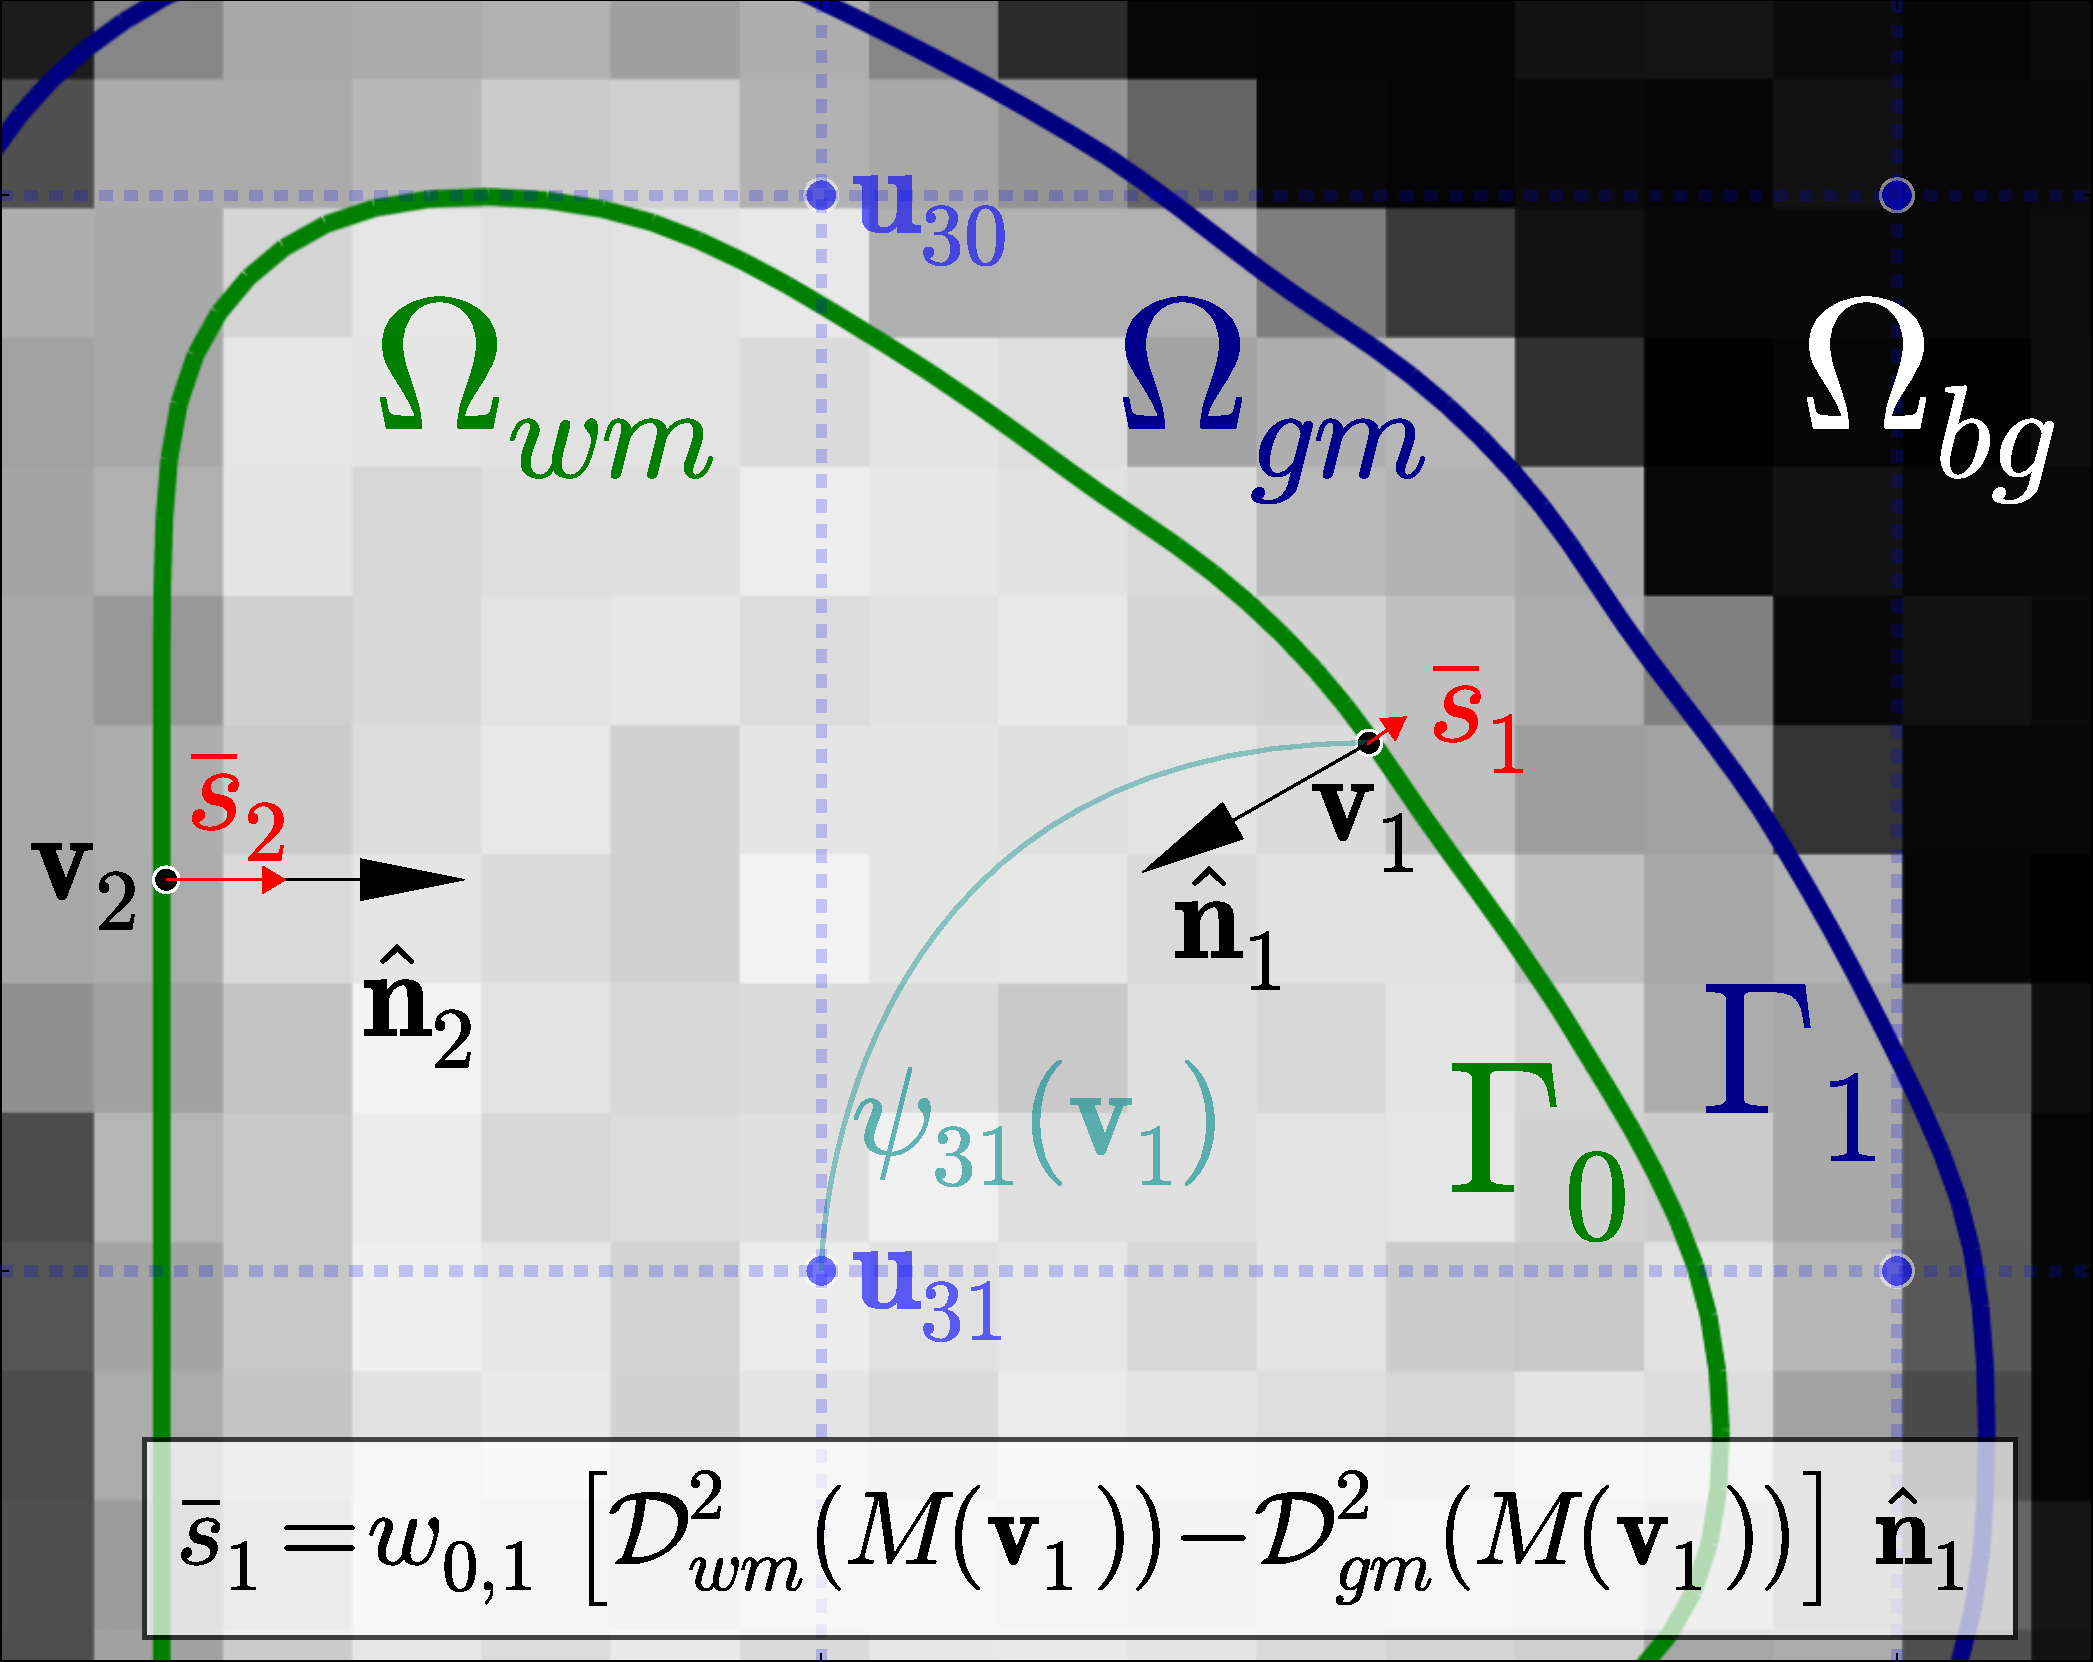
\includegraphics[width=\linewidth]{figures/figure01}
	\caption{The active contours are defined as the interfacing surfaces of the segmenting
	\glspl{roi} $\Omega_i$, and represented in green and dark blue colors in this
	close-up.
	They iteratively through their normals $\hat{n}_i$ at each vertex $\vec{v}_i$ of the mesh.
	The gradient speeds $\bar{s}_i$ are computed as the disparity between data energies of
	the vertex $\vec{v}_i$ in each limiting region as described in \autoref{eq:energy}.
	In this figure, the gradient speed corresponding to $\vec{v}_1$ is written in the lower
	box, $\Omega_{wm}$ being the inner limiting region and $\Omega_{gm}$ the outer.
	Finally, every $\bar{s}_i$ is projected into the grid of control points $\vec{u}_k$ that
	support the deformation field through the corresponding weights $\psi_k(\vec{v}_i)$ obtained
	as in \autoref{eq:basis_derivative}.
	}\label{fig:method}
\end{figure}

\subsubsection{Deformation model}
\label{sec:deformation_model}
Let us denote $\{\vec{v}_i\}_{i=1 \ldots N_c}$ the vertices of one or several prior
  surface(s).
In our application, these surfaces are triangularized meshes extracted using \emph{FreeSurfer}
  \citep{fischl_freesurfer_2012}.
The transformation from the structural space into the coordinate space of the
  target image is achieved through a dense deformation field $u(\vec{r})$, such that:
  \begin{equation}
  \vec{v}_i' = U\{\vec{v}_i\} = \vec{v}_i + u(\vec{v}_i),
  \label{eq:nodes_tfm}
  \end{equation}
  where $U$ is defined in \eqref{eq:transform}.
Since the nodes of the anatomical surfaces likely lay off-grid, it is required to
  derive $u(\vec{r})$ from a discrete set of parameters $\{\vec{u}_k\}_{k=1 \ldots K}$.
Densification is achieved through a set of associated basis functions $\psi_k$:
  \begin{equation}
  u(\vec{r}) = \sum_k \psi_k(\vec{r}) \vec{u}_k.
  \label{eq:intp_kernel}
  \end{equation}
%
In our implementation, $\psi_k$ is chosen to be a tensor-product B-Spline kernel
  of degree 3 ($B_3$).
Then, introducing \eqref{eq:intp_kernel} into \eqref{eq:nodes_tfm} and replacing
  $\psi$ by the actual kernel function, the transformation writes:
  \begin{equation}
    \vec{v}_i' = \vec{v}_i + \sum_k \left[ \vec{u}_k \, \underset{d}{\prod}
      B_3( (\vec{v}_i - \vec{r}_k) \cdot \hat{\mathbf{e}}_d ) \right],
  \label{eq:transformation}
  \end{equation}
  with $\hat{\mathbf{e}}_d$ being the unitary vector along axis $d$.


\subsubsection{Optimization}
\label{sec:gradient_descent}
To find the minimum of the energy functional \eqref{eq:energy},
  we propose a gradient-descent approach with respect to the underlying
  deformation field through the following \gls*{pde}:
  \begin{equation}
  \frac{\partial u(\vec{r},t)}{\partial t} \propto - \frac{\partial E(\vec{u})}{\partial \vec{u}_k},
  \label{eq:general_gradient_descent}
  \end{equation}
  with $t$ being an artificial time parameter of the contour
  evolution, and $\vec{u}_k$ the parameters supporting the estimate
  $\hat{U}$ of the transformation at the current time point.
Now, we introduce \eqref{eq:energy} in \eqref{eq:general_gradient_descent}:
  \begin{align}
  \frac{\partial E(\vec{u})}{\partial \vec{u}_k} &=
  \frac{ \partial }{\partial \vec{u}_k} \Big\{
  \int_{\Omega} \underset{l}{\sum} \mdist{f'}{l} \,d\vec{r} \notag\\
  &+ \int_{\Omega} [ \boldsymbol{\alpha} \cdot u(\vec{r})^{\circ2}
  + \boldsymbol{\beta} \cdot (\nabla \cdot u(\vec{r}))^{\circ2} ] \,d\vec{r}
  \Big\}.
  \label{eq:gradient_descent}
  \end{align}

Therefore, we can apply a discretized interpretation of \eqref{eq:shape_gradients}
  to compute the data term in \eqref{eq:gradient_descent} as follows:
  \begin{align}
  \frac{\partial E_{data}(\vec{u})}{\partial \vec{u}_k} &=
  \frac{ \partial }{\partial \vec{u}_k} \left\{
   \underset{\vec{x} \in \Omega_l}{\sum} \underset{l}{\sum} \mdist{f'}{l} \right\}
  = \underset{i}{\sum}
   \left\langle \frac{\partial \vec{v}_i'}{\partial \vec{u}_k}, \bar{s}_i'\right\rangle,
  \label{eq:gradient_wshape}
  \end{align}
  in this case, the formulation has been adapted to the non-binary case, $\{l,m\}$
  being any pair of neighboring regions, and $\Gamma_{l,m}$ the contour separating
  them such that $\vec{x}' = \vec{v}' \in\Gamma_{l,m} \iff \vec{x}\in \partial\Omega_i \cap \partial\Omega_j$
  and $\vec{n_i}'$ is the unit inward normal to the contour at $c_i'$.

Finally, we can compute:
  \begin{align}
  \frac{\partial \vec{v}_i'}{\partial \vec{u}_k} &= \frac{\partial}{\partial \vec{u}_k}
  \left\{ \vec{v}_i + \sum_k \psi_k(\vec{v}_i) \vec{u}_k \right\}
  = \psi_k(\vec{v}_i)\, \hat{\vec{e}}
  \label{eq:basis_derivative}
  \end{align}
  where $\hat{\vec{e}}$ is the coordinates system's unit vector.
The vertex speeds $\bar{s}_i'$ obtained by computing the shape-gradients \autoref{eq:shape_gradients},
	are then projected to the deformation field in order to obtain the derivatives $\vec{g}_k$
	corresponding to $\vec{u}_k$:
  \begin{equation}
  \vec{g}_{i,k} = \left\langle \frac{\partial}{\partial \vec{u}_k}{\vec{v}_i}', \bar{s}_i'\right\rangle
  = - \left[ \mdist{f_i'}{l} - \mdist{f_i'}{m} \right] \psi_k(\vec{v}_i)\, \hat{\vec{e}},
  \end{equation}
  then the full gradient evolution equation \eqref{eq:gradient_descent} yields:
  \begin{align}
  \frac{\partial E(\vec{u}_k)}{\partial \vec{u}_k} =
  &\underset{i}{\sum} \vec{g}_{i,k} +2\, \boldsymbol{\alpha} \vec{u}_k
  -2\, \boldsymbol{\beta} \Delta \vec{u}_k,
  \label{eq:gradient_final}
  \end{align}



\subsection{Experiments and evaluation}
\label{sec:experiments_evaluation}
%
The experiments follow a five-steps design:
\begin{enumerate}
	\item The prior surfaces are extracted from an undistorted and high-resolution dataset
	  (e.g. \autoref{fig:phantom}).
	\item A plausible, synthetic distortion $U^{-1}_{true}$ is generated.
	\item The low-resolution (target) images are warped using the synthetic distortion.
	\item Our method is run, obtaining a $\hat{U}_{tst}$.
	  A cross-comparison methodology is also applied, to obtain a competing $\hat{U}_{cc}$.
	\item Results are visually and quantitatively evaluated.
\end{enumerate}

To quantitatively evaluate the registration results we computed the \gls*{swindex} as the one-to-one
  distance between corresponding vertices of surfaces, weighted by their respective
  Voronoi area $w_i$:
  \begin{equation}
  sWI = \frac{1}{P} \sum\limits_p^P \frac{1}{A_p} \sum\limits_i^{N_p} w_i\,\|
  \vec{v}_i - \hat{\vec{v}}_i \|
  \end{equation}
  where $\vec{v}_i$ are the locations of the $N_p$ vertices in each $p \in \{1, \dots P\}$
    prior, $A_p$ the total area of surface $p$, and $\hat{\vec{v}}_i$ is the location
    recovered corresponding to the vertex $\vec{v}_i$.

In the application on real data, three experts blindly rated correction results obtained
  with the proposed method and the cross-comparison reference.
The full report of visual results is provided within the Supplemental Materials.

  % \item \gls{wi}, L2-distance between the theoretical and the recovered
  %   deformation field.
  %   \begin{equation}
  %   WI = \frac{1}{N} \sum\limits_i^N \| \mathbf{d}_i - \hat{\mathbf{d}}_i \|
  %   \end{equation}
  %   where $\mathbf{d}_i$ is the theoretical displacement vector at position $i$
  %   and $\hat{\mathbf{d}}_i$ is the recovered one at the same index position.
  % \item Parcellation agreement, the Dice overlap index of the \glspl*{roi}
  %   contained by the parcellation.
  % \end{itemize}



\subsection{Image Data and preprocessing}
\label{sec:datasets}

\subsubsection{Simulated digital phantom} %
\label{sec:digital_phantoms}
%
We first present the proof of the concept on a simplistic digital phantom
  (\autoref{fig:phantom}).
Using \cite{caruyer_phantomas_2014}, we simulated 2.0mm isotropic \gls*{t1} and
  \gls*{t2} images at several rician noise levels, with parameters TE/TR=10/1500ms
  and TE/TR=90/5000ms respectively.
The reference surfaces were extracted using the marching-cubes algorithm
  shipped with \emph{FreeSurfer} \citep{fischl_freesurfer_2012}
  on high-resolution (1.0mm isotropic) and binary images corresponding to
  the tissue fraction maps used in simulations.

\begin{figure}
	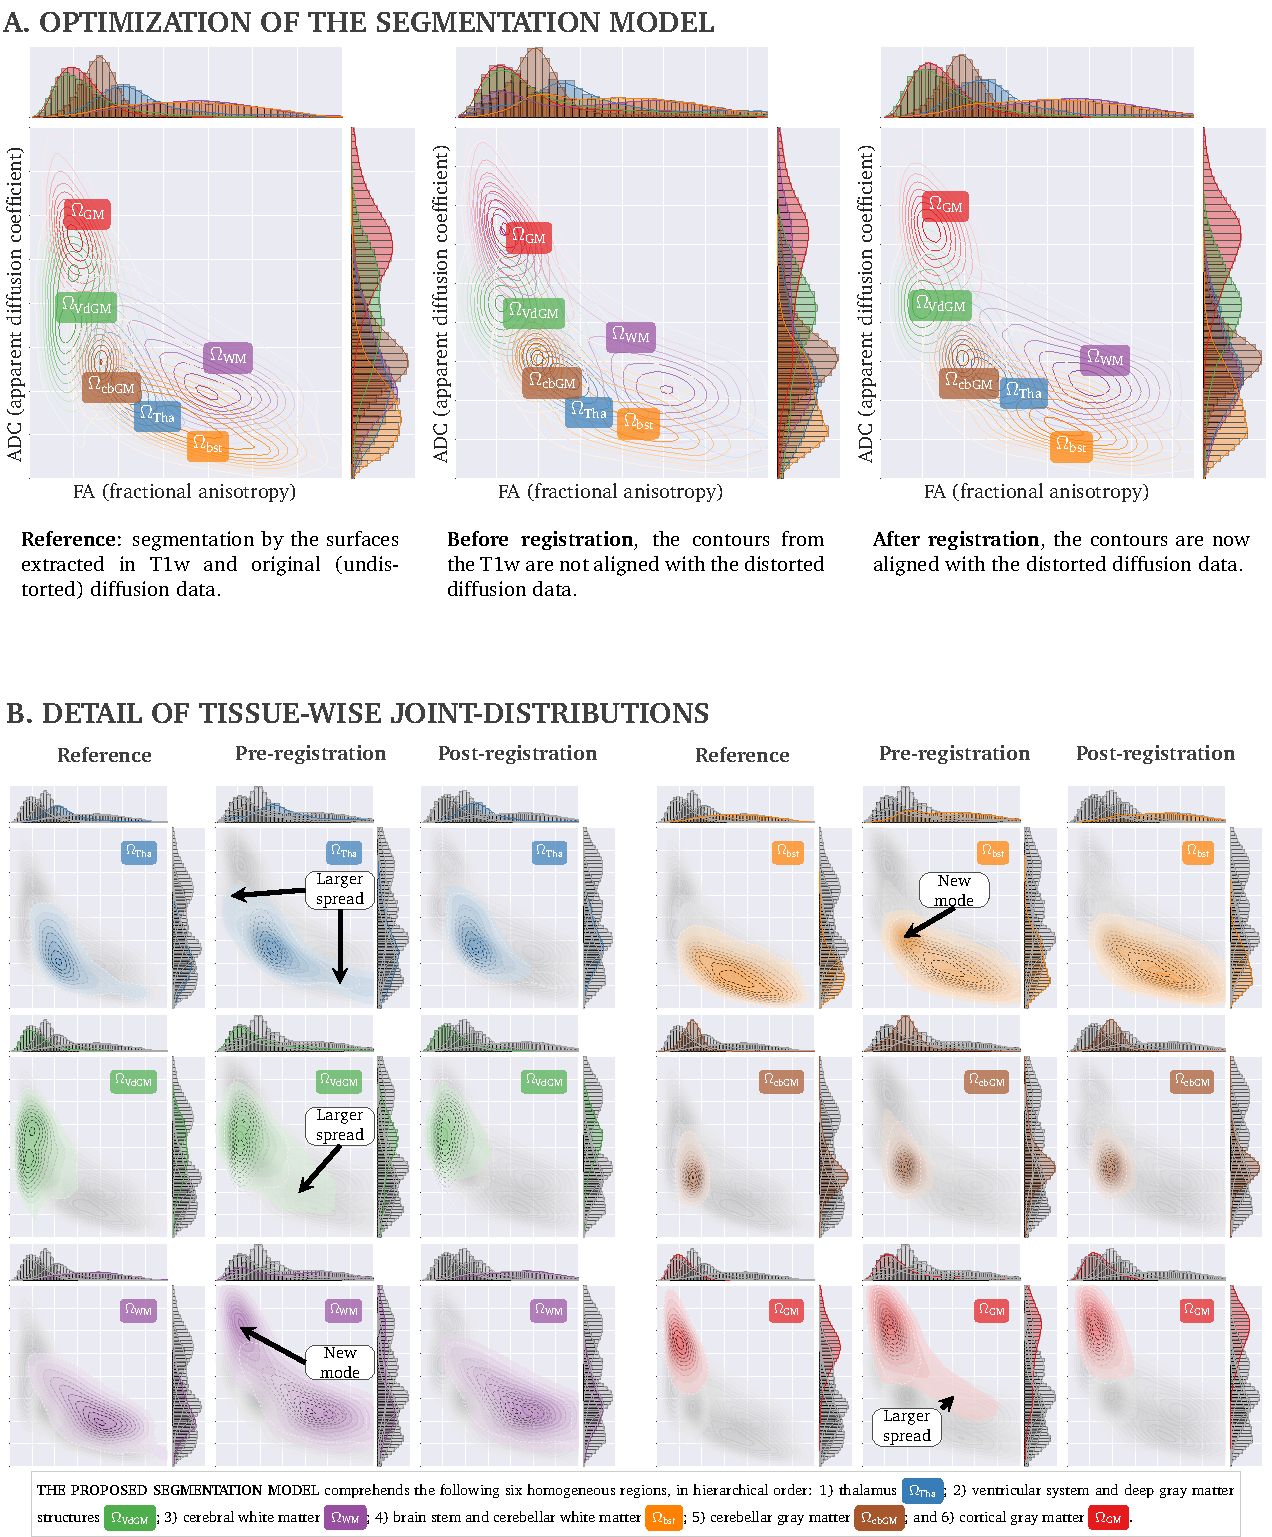
\includegraphics[width=\linewidth]{figures/figure02}
	\caption{The ``cortex'' phantom is a spherical shape with two sulci and an
	 outer crust resembling the cortical folding.
	When the model is used to generate low resolution images, the
	  partial volume effect turns segmentation of the sulci a
	  challenging problem with voxel-wise clustering methods,
	  but it is successfully segmented with the proposed method (see
	  \autoref{fig:results_phantom}).
	Top row shows the central-axial plane of the simulated images at
	  high resolution and noiseless (left is \gls*{t1} and right is
	  \gls*{t2}).
	Bottom row represents the extracted contours that are used as shape
	  priors to be registered to low-resolution, noise corrupted versions
	  of the phantom.
	}\label{fig:phantom}
\end{figure}

\subsubsection{Real \gls{mri} datasets} %
\label{sec:human_connectome}
%
For the evaluation of the algorithm to real \gls*{dmri} data of human brains,
  we downloaded 10 datasets from the ``minimally preprocessed''
	 database of the \gls*{hcp}.
We refer the reader to \citep{essen_human_2012} for exact details about acquisition
  parameters, and \citep{glasser_minimal_2013} for preprocessing issues.
The datasets comprehend \gls*{t1}, \gls*{t2} and multi-shell \gls*{dmri} images
  already corrected for artifacts, brain-extracted and spatially normalized,
  along with the most prominent results of the standard processing with
  \emph{FreeSurfer}: \emph{aparc} segmentations, and the surfaces corresponding to
  the cortical \gls*{gm} exterior and the \gls*{wm} interface with
  cortical \gls*{gm}.
